\documentclass{llncs}

%\usepackage{llncsdoc}

%\usepackage{makeidx}  % allows for indexgeneration
\usepackage{graphicx}
\usepackage[T1]{fontenc}
\usepackage[english]{babel}
\usepackage[utf8]{inputenc}

\usepackage{paralist}


%%%Math
\usepackage{latexsym}
\usepackage{amsmath}
\usepackage{amssymb}
\usepackage{amsthm}

\usepackage{algorithm}
\usepackage{algorithmic}

\usepackage{longtable}

\usepackage{listings}

\usepackage{color}

\definecolor{darkred}{rgb}{0.5, 0, 0}
\definecolor{violet}{rgb}{1, 0, 1}
\definecolor{green}{rgb}{0.3, 0.95, 0.3}
\definecolor{listinggray}{gray}{0.97}

\lstset{
	basewidth=0.45em,
	backgroundcolor=\color{listinggray},
	basicstyle=\footnotesize\ttfamily,
	breaklines=true,
	keywordstyle=\bfseries,
	stringstyle=\itshape,
	commentstyle=\itshape,
	showspaces=false,
	showtabs=false,
	showstringspaces=false,
	frame=trbl,
	frameround=tttt,
	extendedchars=true,
	numbers=none,
	aboveskip=0.5cm,
	belowskip=0.5cm,
	xleftmargin=0cm,
	xrightmargin=0cm
}


\begin{document}

\title{Application of the Spreading Activation Technique for Recommending Concepts of well-known ontologies in Medical Systems}

\titlerunning{Application of the Spreading Activation Technique for Recommending Concepts of well-known ontologies in Medical Systems}

\author{Jose Mar\'{i}a \'{A}lvarez\inst{1} \and Pablo Abella\inst{1} \and Weena Jimenez\inst{1} \and Jos\'{e} Emilio Labra\inst{1}} 


\authorrunning{Jose Mar\'{i}a Alvarez et al.}


\tocauthor{Jose Mar\'{i}a \'{A}lvarez, Diego Berrueta, Luis Polo, Jos\'{e} Emilio
Labra} 


\institute{WESO RG, Universidad de Oviedo, Oviedo, Asturias, Spain,\\
\email{\{josem.alvarez,pablo.abella,weena.jimenez,jelabra\}@weso.es},\\ 
 WWW home page: \texttt{http://www.weso.es}
}

\maketitle

\begin{abstract}
The present paper introduces the ONTOSPREAD framework for the development,
configuration, customization and execution of the Spreading Activation
technique over graph-based structures, more specifically over RDF graphs and ontologies 
arising from the Semantic Web area. This technique has been used to
the efficient exploration and querying of large and heterogeneous knowledge bases 
based on semantic networks in the Information and Document Retrieval domains. 
ONTOSPREAD implements the double process of activation and spreading of concepts in ontologies applying 
different restrictions of the original model like weight degradation according to the distance or 
others coming from the extension of this technique like the converging paths reward. 
This technique provide a whole framework to ease the information access, 
common required feature in the exploitation of new and existing digital libraries. 
Finally an evaluation methodology and an example using the Galen ontology 
are provided to validate the goodness, the improvement and the capabilities of this framework applied 
to digital libraries.
\end{abstract}

% The main application of Spreading Activation
% lies in two different areas of interest to digital libraries: 1) construction of hybrid semantic search engines 2) ranking of
% information resources according to an input set of weighted resources.

\section{Introduction}
\input{sections/intro}
\section{Related Work}\label{related-work}
Since SA was introduced by~\cite{Collins_Loftus_1975} in the field of 
psycho linguistics and semantic priming it has been applied to the resolution
of problems trying to simulate the behavior of the brain using a connectionist method
to provide an ``intelligent'' way to retrieve information and data. 

The use of SA was motivated due to the research on graph exploration~\cite{Scott1981}. Nevertheless
the success of this technique is specially relevant to the fields of Document~\cite{turtle91inference} 
and Information Retrieval~\cite{Cohen1987}. It has
been also demonstrated its application to extract correlations between query terms and documents analyzing user 
logs~\cite{Cui03} and to retrieve resources amongst multiple systems~\cite{Schumacher+2008search} 
in which ontologies are used to link and annotate resources.

In recent years and regarding the emerging use of ontologies in the Semantic Web area new applications of SA have
appeared to explore concepts~\cite{Qiu93,Chen95} addressing the two important issues: 1) the selection and 2) the weighting of
additional search terms and to measure conceptual similarity~\cite{gouws-vanrooyen-engelbrecht:2010:CCSR}. 
On the other hand, there are works~\cite{DBLP:journals/cogsr/KatiforiVD10} 
exploring the application of the SA on ontologies in order to create context inference models.The 
semi-automatically extension and refinement of ontologies~\cite{liu_et_al_2005} is other trending topic to apply SA
in combination with other techniques based on natural language processing. Data mining,
more specifically mining socio-semantic networks\cite{paper:troussov:2008}, and applications 
to collaborative filtering (community detection based on tag recommendations, expertise location, etc.) are other 
potential scenarios to apply the SA theory due to the high performance and high scalability of the technique. In particular, 
annotation and tagging~\cite{labraTagging2007} services to gather meta-data~\cite{GelgiVD05} from the Web or to predict social annotation~\cite{Chen:2007:PSA:1780653.1780702} and recommending 
systems based on the combination of ontologies and SA~\cite{citeulike:3779904} are taken advantage of using SA technique. 
Also the semantic search~\cite{conf-sofsem-Suchal08} is a highlight area to apply SA following
hybrid approaches~\cite{bopaEstonia,RochaSA04} or user query expansion~\cite{767402} combining metadata 
and user information.

Although this technique is widely accepted and applied to different fields open implementations\footnote{ 
Texai company~(\url{http://texai.org/}) offers a proprietary implementation of SA.}, are missing. Moreover 
the Apache Mahout~\footnote{\url{http://mahout.apache.org/}} project, a recent scalable machine learning library 
that supports large data sets, does not include an implementation of SA instead of 
providing algorithms for the classification, clustering, pattern mining, 
recommendation and collaborative filtering of resources in which SA should be representative. 
 



\section{ONTOSPREAD Framework}
\subsection{Background}\label{background}
In this section, the theoretical model of \textit{SA}~\cite{Collins_Loftus_1975,AndersonTheory} is reviewed to 
illustrate the basic components and the operations performed by SA during their execution, specially
the spread of the activation from a node to their adjacent, see Fig.~\ref{fig:spreading}. 
This model is made up of a conceptual network of nodes connected through relations (conceptual graph). 
Taking into account that nodes represent domain objects or classes and edges relations among them, 
it is possible to establish a semantic network in which SA can be applied. The process performed by the algorithm 
is based on a thorough method to go down the graph using an iterative model. Each iteration is comprised of 
a set of beats, a stepwise method, and the checking of a stop condition. 
Following the different stages of SA are presented and defined:

\begin{figure}[h]
 \centering
    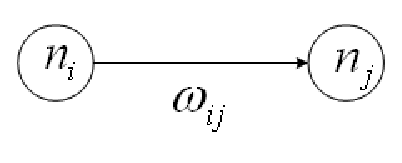
\includegraphics[width=3cm]{images/spreading}
    \caption{Graphical model of \textit{Spreading Activation}}
 \label{fig:spreading}
\end{figure}

\begin{description}
\item [\textit{Preadjustement}:] This is the initial and optional stage. It is usually in charge
of performing some control strategy over the target semantic network.
\medskip

\item [\textit{Spreading}:] This is the spread stage of the algorithm. Concepts
are activated in activation waves. The spreading node activates its neighbor
nodes, see Fig.~\ref{fig:modelo-sa}.
\medskip

The calculation of the activation rank $I_i$ of a node $n_i$ is defined as
follows:

\begin{equation}
I_i  = \sum_j{O_j \omega_{ji}}
\end{equation}
\medskip

$I_i$ is the total inputs of the node $n_i$, $O_j$
is the output of the node $n_j$ connected to $n_i$ and $\omega_{ji}$
is the weight of the relation between $n_j$ and $n_i$. 
If there is not relation between $n_j$ and $n_i$ then
$\omega_{ji} = 0$. 


The activation function $f$ is used to evaluate the ``weight'' of a node and
decide if the concept is active.


\begin{equation}
N_i=f(I_i)=\begin{cases} 0 & \text{if $I_i < \jmath_i$} \\ 1 &
\text{if $I_i > \jmath_i$}
\\ \end{cases}
\end{equation}


$N_i$ is $1$ if the node has been activated or 0 otherwise. 
$\jmath_i$, the threshold activation value for node $i$, depends on the application
and it can change from a node to others. The activation rank $I_i$ of a
node $n_i$ will change while algorithm iterates.

\begin{figure}[h]
 \centering
 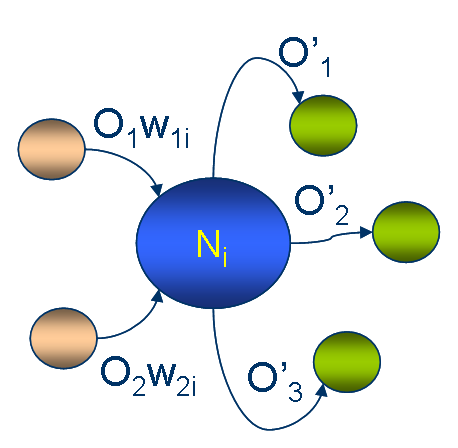
\includegraphics[width=4cm]{images/modelo-sa}
    \caption{Activation of concepts in \textit{Spreading Activation}}
 \label{fig:modelo-sa}
\end{figure}

\item [\textit{Postadjustment}:] This is the final and optional stage. As well as
\textit{Preadjustment} stage, it is used to perform some control strategy in the
set of activated concepts.

\end{description}

\input{sections/sa}
\section{Evaluation of ONTOSPREAD}
\subsection{ONTOPSREAD API in Action}
\section{Conclussions and Future Work}
\input{sections/conclussions}


\bibliographystyle{plain}
% %\bibliographystyle{unsrt}
% %\bibliographystyle{acm}
\bibliography{bib/references}
% \renewcommand{\bibname}{References}
\end{document}
